\chapter{Introduction}
\label{ch:intro}

\section{Background of Industrial Attachment}
\label{sec:background}

Brain Station 23 (BS-23) is a renowned software development company based in Dhaka, Bangladesh, specializing in custom software solutions, full-stack web and mobile development, cloud-native architecture, and AI integration. BS-23 was selected for this industrial attachment based on three principal criteria: (i) a demonstrated track record of implementing modern software engineering practices including Agile Scrum, CI/CD, and microservices architecture; (ii) expertise in full-stack JavaScript/TypeScript ecosystems aligned with current academic and industry curricula; and (iii) a structured internship mentorship program with senior engineers actively guiding junior developers.

BS-23 operates across healthcare, e-commerce, logistics, fintech, and hospitality domains, serving both domestic and international clients. Their project portfolio consistently demonstrates application of rigorous engineering principles to solve real business problems --- making the organization an ideal environment for bridging academic knowledge with professional practice.

The attachment was conducted from \textbf{23 February to 6 March 2026} (10 working days), with project kickoff and team formation beginning 20 February 2026\footnote{BS-23 attachment formally counts 10 working days, excluding Friday--Saturday weekends. Initial onboarding, proposal selection, and repository bootstrap occurred 20--22 Feb.}. The attachment site provided a realistic corporate engineering environment: daily Scrum stand-ups, GitHub-based code review, mentor feedback sessions, and a final stakeholder presentation.

\textbf{Attachment Context.} The assigned vehicle was \textbf{neoRMS --- AI-Integrated Restaurant Management System} --- a multi-tenant, real-time restaurant operations platform. The project presented a genuine full-stack engineering challenge: multi-role authentication, real-time order orchestration via WebSockets, payment integration, inventory management, and AI-driven analytics --- making it an ideal vehicle for achieving program outcomes in system architecture, distributed systems, and team leadership.

\section{Importance in Achieving Engineering Program Outcomes}
\label{sec:po}

The industrial attachment at BS-23 directly contributes to six key engineering program outcomes defined by the CSE, RUET Outcome-Based Education framework:

\begin{itemize}
\item \textbf{Real-world Problem Solving (PO1, PO2):} Translating ambiguous restaurant operations requirements into a normalized database schema, REST + WebSocket API contracts, and a deployable system.
\item \textbf{Technical Implementation (PO3, PO5):} Hands-on design and implementation of authentication (JWT + RBAC), WebSocket multi-namespace architecture, Prisma ORM data modeling, Docker containerization, and AI service bridging.
\item \textbf{Project Management (PO11):} Serving as Backend Team Lead --- sprint planning, API contract negotiation between frontend/backend, task allocation, code review of 23 pull requests, and risk mitigation under a 10-day deadline.
\item \textbf{Teamwork \& Communication (PO9, PO10):} Coordinating a 7-member cross-functional team (3 backend, 3 frontend, 1 AI), facilitating daily stand-ups, resolving integration conflicts, and delivering a unified stakeholder presentation.
\item \textbf{Professional Ethics (PO8):} Handling user PII, payment data, secure credential management, intellectual property compliance, and IEEE Code of Ethics application in real tasks.
\item \textbf{Industry Standards \& Lifelong Learning (PO12):} Exposure to Express 5, Prisma 6, Socket.IO 4, Swagger/OpenAPI, Docker Compose, GitHub Actions, and self-directed learning of WebSocket scaling patterns and AI service integration.
\end{itemize}

\begin{figure}[H]
\centering
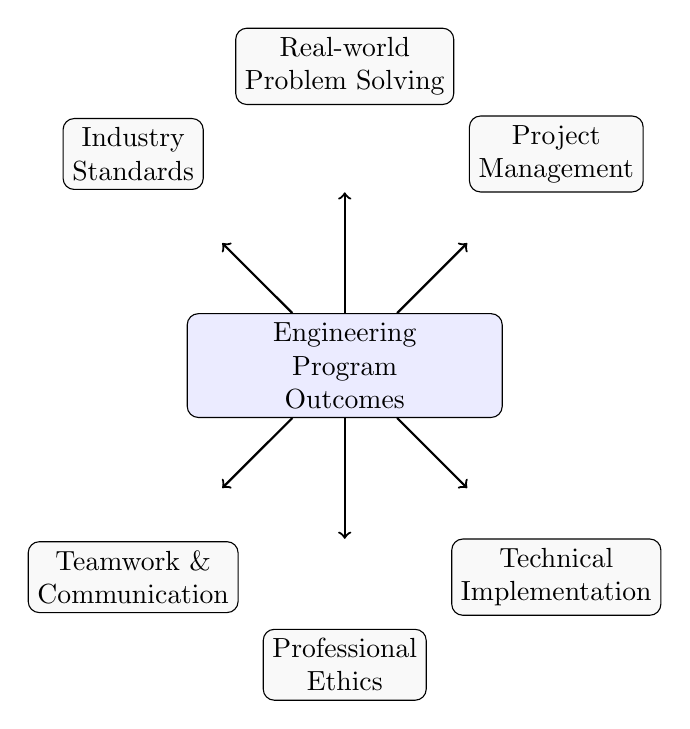
\begin{tikzpicture}
\node[draw,rounded corners,align=center,minimum width=4cm,minimum height=1.2cm,fill=blue!8] (center) at (0,0) {Engineering\\Program\\Outcomes};
\foreach \a/\t in {90/Real-world\\Problem Solving,45/Project\\Management,-45/Technical\\Implementation,-90/Professional\\Ethics,-135/Teamwork \&\\Communication,135/Industry\\Standards} {
  \node[draw,rounded corners,align=center,fill=gray!5] at (\a:3.8cm) {\t};
  \draw[->,thick] (center) -- (\a:2.2cm);
}
\end{tikzpicture}
\caption{Engineering Program Outcomes Addressed by the Attachment}
\label{fig:po}
\end{figure}

\section{Objectives of the Attachment}
\label{sec:objectives}

The primary objectives were:

\begin{enumerate}
\item To gain practical exposure to real-world, full-stack software development workflows, with emphasis on system architecture and technical leadership.
\item To design and implement a scalable backend architecture including authentication, multi-tenant data isolation, and real-time WebSocket communication.
\item To understand and apply Agile Scrum in a time-boxed, high-velocity professional project environment.
\item To develop hands-on skills in Node.js / Express 5, PostgreSQL, Prisma ORM, Socket.IO, Docker, and AI service integration via FastAPI.
\item To lead a cross-functional engineering team --- including task decomposition, API contract definition, code review, and mentorship of less-experienced developers.
\item To apply theoretical knowledge from Database Systems, Software Engineering, Computer Networks, and System Analysis \& Design courses to production-grade scenarios.
\item To experience professional responsibility, ethical conduct, technical documentation standards, and stakeholder presentation in software engineering.
\end{enumerate}

\section{Scope and Limitations}
\label{sec:scope}

\subsection{Scope}

\begin{table}[H]
\centering
\caption{Scope of the Industrial Attachment}
\label{tab:scope}
\begin{tabularx}{\textwidth}{@{}p{0.28\textwidth}X@{}}
\toprule
\textbf{Scope Area} & \textbf{Description} \\
\midrule
System Architecture & End-to-end architecture design: 3-tier + WebSocket realtime layer + AI service bridge. Database schema (22 entities, 3NF), API contract design, project bootstrap. \\
Backend Leadership & Backend Team Lead: auth \& RBAC, WebSocket server (3 namespaces), order core, reservation API, AI integration, deployment (Docker), code review. \\
Real-time Engineering & Socket.IO multi-namespace, room-based tenant isolation, event-driven order state machine: customer $\rightarrow$ waiter $\rightarrow$ chef $\rightarrow$ customer. \\
AI Integration & Bridging Python FastAPI AI microservice: recommendation engine, sentiment analysis, review analyzer --- REST bridge with retry \& fallback. \\
DevOps & Docker-first strategy: \texttt{Dockerfile}, \texttt{compose.yaml}, environment parity for frontend team zero-setup onboarding. \\
Project Management & Agile Scrum: sprint planning, daily stand-ups, API-first contracts, PR review (23 PRs), cross-team coordination, final presentation delivery. \\
\bottomrule
\end{tabularx}
\end{table}

\subsection{Limitations}

\begin{table}[H]
\centering
\caption{Limitations of the Industrial Attachment}
\label{tab:limitations}
\begin{tabularx}{\textwidth}{@{}p{0.28\textwidth}X@{}}
\toprule
\textbf{Limitation} & \textbf{Implication} \\
\midrule
10-day duration & Restricted scope for comprehensive E2E testing, performance benchmarking, and production hardening. MVP prioritized over edge-case completeness. \\
Incomplete feature set & Advanced features (deposit refund logic, push notifications, 24-hr reminder cron, email service) scoped out --- marked OUT OF SCOPE in backlog. \\
Limited production access & Deployment limited to Docker staging; restricted exposure to full CI/CD, Kubernetes, and cloud autoscaling procedures at BS-23. \\
Team experience variance & 6 of 7 team members were first-time full-stack project contributors; significant mentoring overhead reduced individual deep-technical velocity. \\
Proprietary information & Certain BS-23 internal tooling, client data, and HR processes are confidential and excluded per NDA. \\
\bottomrule
\end{tabularx}
\end{table}

\section{Methodology}
\label{sec:methodology}

The attachment followed a structured, iterative Agile Scrum methodology, adapted for a 10-day hyper-sprint:

\textbf{Requirements Collection $\rightarrow$ Architecture Design $\rightarrow$ API Contract First $\rightarrow$ Parallel Implementation $\rightarrow$ Integration $\rightarrow$ Testing $\rightarrow$ Documentation $\rightarrow$ Presentation}

Data collection for this report included: direct participation logs, Git commit history (141 commits authored), daily stand-up notes, pull request review comments (23 PRs reviewed/merged), mentor feedback sessions, and peer retrospectives. Documentation was maintained concurrently via GitHub README, Swagger annotations, and daily log sheets --- ensuring traceability.

\begin{figure}[H]
\centering
\begin{tikzpicture}[node distance=1.8cm, every node/.style={draw,rounded corners,align=center,minimum width=2.4cm,minimum height=0.9cm,fill=blue!5}]
\node (r) {Requirements\\Collection};
\node[right=of r] (d) {Design\\Phase};
\node[right=of d] (i) {Implementation};
\node[right=of i] (t) {Integration\\\& Testing};
\node[right=of t] (doc) {Documentation\\\& Presentation};
\draw[->,thick] (r) -- (d);
\draw[->,thick] (d) -- (i);
\draw[->,thick] (i) -- (t);
\draw[->,thick] (t) -- (doc);
\draw[->,thick,dashed] (doc) to[bend left=20] node[above,draw=none,fill=none]{iterative} (r);
\end{tikzpicture}
\caption{Attachment Methodology --- Development Lifecycle}
\label{fig:methodology}
\end{figure}

\section{Attachment Timeline}
\label{sec:timeline}

\begin{table}[H]
\centering
\small
\caption{Industrial Attachment Timeline --- Day-by-Day Overview (Backend Team Lead)}
\label{tab:timeline}
\begin{tabularx}{\textwidth}{@{}p{0.10\textwidth}p{0.18\textwidth}X@{}}
\toprule
\textbf{Day(s)} & \textbf{Focus Area} & \textbf{Key Activities --- Naimuzzaman} \\
\midrule
Day 0 \newline 20--22 Feb & Proposal \& Bootstrap & Team formation (7 members), project proposal defense --- neoRMS selected. GitHub mono-repo + submodules initialized. Database ERD v1, project structure scaffold, \texttt{Dockerfile} + \texttt{compose.yaml} committed. Prisma setup. \\
Day 1 \newline 23 Feb & Onboarding \& Architecture & BS-23 onboarding, Scrum introduction, SRS/BRD drafting. Auth module bootstrap: JWT access/refresh, RBAC middleware, tenant middleware. Schema finalization (22 entities). \\
Day 2 \newline 24 Feb & Auth \& Core APIs & JWT Authentication Endpoints (BE-001) merged. RBAC Middleware (BE-002) merged. Restaurant context / pagination utils. Code review: Staff Account APIs (Saim). \\
Day 3 \newline 25--26 Feb & Order Core \& WebSocket & Order Placement Endpoint (BE-005). WebSocket Server \& Room Management (BE-017): 3 namespaces --- \texttt{/waiter}, \texttt{/chef}, \texttt{/customer}. Socket auth middleware. Frontend WebSocket client wiring begins. \\
Day 4 \newline 27 Feb & Integration \& Coupon & Coupon--Order integration, pagination refactor, tenant access validation. Code review: Analytics Endpoints, Promotions CRUD (Saim). Feature diagram finalized. \\
Day 5--6 \newline 2--3 Mar & Reservation \& Order Fix & Table Reservation Availability + Create Endpoints (BE-027/028). Order fix PRs merged (\#15, \#17, \#18). Frontend order flow debugging --- cross-team firefighting. \\
Day 7--8 \newline 4--5 Mar & AI Integration \& Socket Events & AI service bridge: \texttt{modules/aiService} --- sentimentAnalysis, review\_analyzer, getRecommendation, sendOrderData. Review routes + schema update. Socket event emission pipeline: \texttt{emitSocketEvent}. Waiter / Chef portal WebSocket frontend implemented (17 + 15 commits). \\
Day 9 \newline 5 Mar & Review \& Frontend Integration & Review module merge (\#22). Order / table reservation / review frontend integration completed. E2E order test: customer $\rightarrow$ waiter $\rightarrow$ chef $\rightarrow$ customer realtime. \\
Day 10 \newline 6 Mar & AI Finalization \& Presentation & AI recommendations integration PR \#23 merged. Seed data + AI DB population. Final project presentation delivered by Team Lead. Post-demo: cash payment order completion fix. \\
\bottomrule
\end{tabularx}
\end{table}

\noindent\textit{Note:} Official BS-23 attachment counts 10 working days (23 Feb -- 6 Mar), excluding weekends. Pre-attachment bootstrap (20--22 Feb) included proposal defense and repository initialization.

\section{Structure of the Report}
\label{sec:structure}

\begin{table}[H]
\centering
\caption{Report Structure Overview}
\label{tab:report_structure}
\begin{tabularx}{\textwidth}{@{}p{0.22\textwidth}X@{}}
\toprule
\textbf{Chapter} & \textbf{Content} \\
\midrule
Chapter 1 & Introduction: background, engineering program outcomes, objectives, scope, methodology, timeline \\
Chapter 2 & Organization overview of Brain Station 23 \\
Chapter 3 & Detailed project overview of neoRMS --- architecture, modules, database, WebSocket realtime design \\
Chapter 4 & Tools and techniques utilized --- selection criteria, complex problem application \\
Chapter 5 & Societal, health, safety, legal and cultural considerations \\
Chapter 6 & Professional ethics and responsibilities \\
Chapter 7 & Skills gained and lifelong learning --- with leadership transition reflection \\
Chapter 8 & Challenges encountered and solutions implemented \\
Chapter 9 & Contributions to the organization --- Backend Team Lead impact, Impact Summary \\
Chapter 10 & Conclusion and recommendations \\
References & IEEE format \\
Appendices & A: Daily Log Sheet, B: Code Snippets, C: Additional Resources + QR \\
\bottomrule
\end{tabularx}
\end{table}
